\section{Resultados}

\subsection{Conjunto de datos evaluado}

Los experimentos se realizaron sobre la serie de demanda eléctrica de Austria (\texttt{AT}), extraída de Open Power System Data y procesada bajo el contrato \texttt{timestamp}/\texttt{y}. La serie utilizada contiene 50,400 observaciones horarias continuas entre el 1 de enero de 2015 a las 00:00 UTC y el 30 de septiembre de 2020 a las 23:00 UTC, sin valores faltantes, duplicados ni discontinuidades en la frecuencia horaria.

El bloque de entrenamiento de N-BEATS abarcó desde el 1 de enero de 2015 hasta el 31 de diciembre de 2018, lo que corresponde a 35,064 observaciones horarias. A partir de ese entrenamiento, se generaron cuatro pronósticos independientes, uno por cada horizonte, utilizando orígenes de pronóstico determinados por la ventana de entrada requerida. ARIMA fue ajustado para cada horizonte con los últimos 17,520 registros horarios previos a cada origen de pronóstico, equivalentes a dos años de historia. La Tabla~\ref{tab:tramos-evaluacion} resume los tramos de evaluación utilizados.

\begin{table}[htbp]
    \centering
    \caption{Tramos de evaluación por horizonte}
    \label{tab:tramos-evaluacion}
    \begin{tabular}{lrrll}
        \toprule
        Horizonte & Horas & \texttt{input\_size} & Inicio del pronóstico & Fin del pronóstico \\
        \midrule
        Diario & 24 & 168 & 2019-01-08 00:00 UTC & 2019-01-08 23:00 UTC \\
        Semanal & 168 & 672 & 2019-01-29 00:00 UTC & 2019-02-04 23:00 UTC \\
        Bisemanal & 336 & 1344 & 2019-02-26 00:00 UTC & 2019-03-11 23:00 UTC \\
        Mensual & 720 & 2160 & 2019-04-01 00:00 UTC & 2019-04-30 23:00 UTC \\
        \bottomrule
    \end{tabular}
\end{table}

\subsection{Métricas de error por modelo}

Las métricas se calcularon sobre exactamente los mismos timestamps para N-BEATS y ARIMA, garantizando que las diferencias observadas reflejen el comportamiento de cada modelo y no discrepancias en los tramos evaluados. La Tabla~\ref{tab:metricas-modelos} presenta los resultados obtenidos.

\begin{table}[htbp]
    \centering
    \caption{Métricas de error para ARIMA y N-BEATS por horizonte}
    \label{tab:metricas-modelos}
    \begin{tabular}{lrrrrrr}
        \toprule
        & \multicolumn{3}{c}{ARIMA} & \multicolumn{3}{c}{N-BEATS} \\
        \cmidrule(lr){2-4} \cmidrule(lr){5-7}
        Horizonte & MAE & RMSE & MAPE & MAE & RMSE & MAPE \\
        \midrule
        24 h & 281.37 & 306.12 & 3.13\% & 275.98 & 343.68 & 2.96\% \\
        168 h & 603.67 & 789.27 & 7.67\% & 335.39 & 418.00 & 4.21\% \\
        336 h & 499.69 & 743.04 & 7.13\% & 235.35 & 290.54 & 3.09\% \\
        720 h & 842.68 & 1046.87 & 11.60\% & 625.89 & 792.43 & 9.57\% \\
        \bottomrule
    \end{tabular}
\end{table}

En el horizonte diario, ambos modelos presentan un desempeño comparable. El MAE de N-BEATS (275.98 MW) es ligeramente inferior al de ARIMA (281.37 MW), aunque el RMSE de N-BEATS (343.68 MW) es mayor que el de ARIMA (306.12 MW), lo que indica que N-BEATS incurrió en algunos errores puntuales más grandes en este horizonte. El MAPE se mantiene por debajo del 3.2\% para ambos modelos.

En el horizonte semanal, N-BEATS muestra una ventaja clara en las tres métricas. El MAE de N-BEATS (335.39 MW) representa una reducción del 44.4\% respecto al MAE de ARIMA (603.67 MW). El RMSE sigue la misma tendencia, con N-BEATS alcanzando 418.00 MW frente a 789.27 MW de ARIMA. El MAPE de N-BEATS (4.21\%) equivale aproximadamente a la mitad del MAPE de ARIMA (7.67\%).

En el horizonte bisemanal se observa la mayor diferencia relativa entre ambos modelos. Aunque este horizonte duplica la extensión del semanal, las métricas de N-BEATS (MAE 235.35 MW, RMSE 290.54 MW, MAPE 3.09\%) son incluso mejores que las obtenidas en el horizonte anterior, lo que sugiere que las condiciones de la serie durante el tramo evaluado (finales de febrero e inicios de marzo) favorecieron la predicción. ARIMA, en contraste, mantiene errores elevados (MAE 499.69 MW, RMSE 743.04 MW, MAPE 7.13\%), consistentes con la dificultad que representa este alcance temporal para los modelos puramente estadísticos.

En el horizonte mensual, ambos modelos experimentan la mayor degradación de desempeño. El MAE de N-BEATS asciende a 625.89 MW y su MAPE a 9.57\%, mientras que ARIMA alcanza un MAE de 842.68 MW y un MAPE de 11.60\%. A pesar del aumento general del error, N-BEATS mantiene una ventaja del 25.7\% en MAE y del 17.5\% en MAPE respecto a ARIMA. Este resultado es consistente con la dificultad inherente de predecir 720 horas hacia adelante a partir únicamente de la trayectoria histórica de la demanda, sin información exógena.

La Figura~\ref{fig:forecast-series} muestra los pronósticos de ambos modelos contra los valores reales para cada horizonte, incluyendo una ventana de contexto histórico que permite apreciar visualmente la continuidad entre la serie de entrada y el pronóstico generado.

\begin{figure}[htbp]
    \centering
    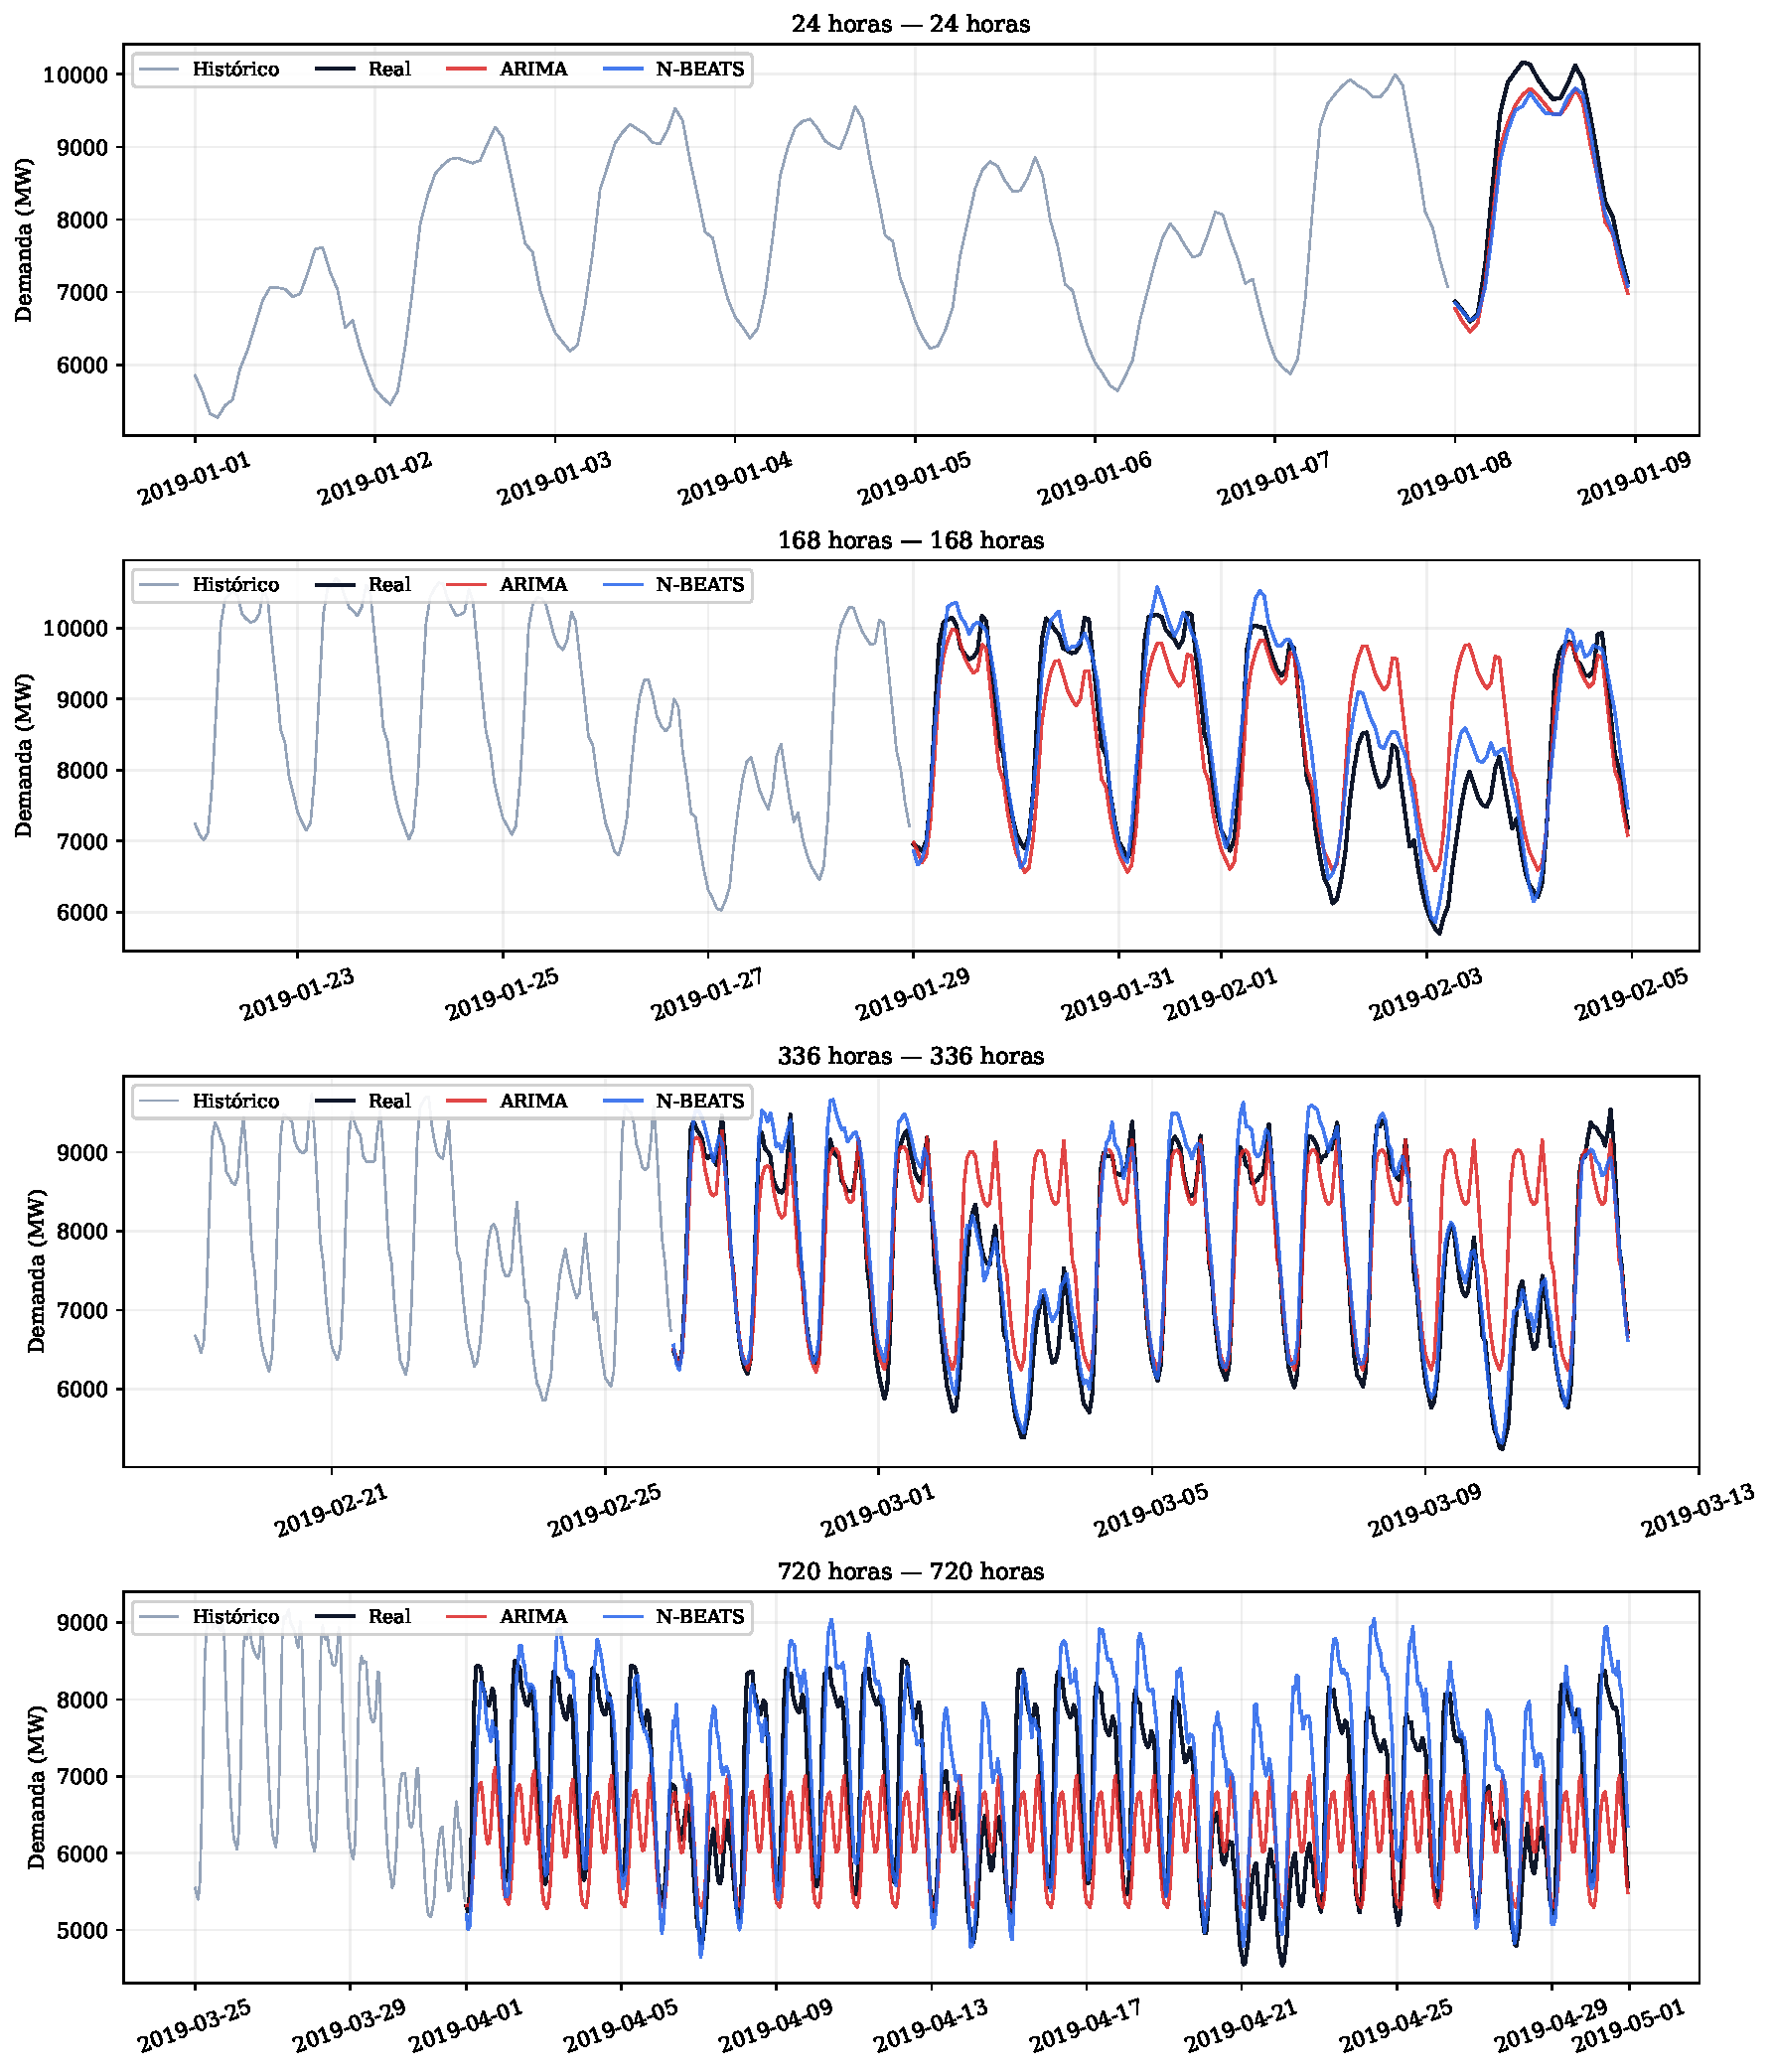
\includegraphics[width=\textwidth]{figures/forecast_time_series.pdf}
    \caption{Pronósticos de ARIMA y N-BEATS contra valores reales por horizonte. La zona sombreada en gris corresponde al contexto histórico utilizado como entrada del modelo N-BEATS.}
    \label{fig:forecast-series}
\end{figure}

La Tabla~\ref{tab:comparacion-relativa} resume la diferencia relativa de N-BEATS respecto a ARIMA, donde valores negativos indican menor error de N-BEATS. La Figura~\ref{fig:metrics-bars} complementa esta comparación con una visualización de barras agrupadas por métrica y horizonte.

\begin{table}[htbp]
    \centering
    \caption{Diferencia relativa de N-BEATS respecto a ARIMA}
    \label{tab:comparacion-relativa}
    \begin{tabular}{lrrr}
        \toprule
        Horizonte & $\Delta$ MAE & $\Delta$ RMSE & $\Delta$ MAPE \\
        \midrule
        24 h & $-$1.9\% & $+$12.3\% & $-$5.4\% \\
        168 h & $-$44.4\% & $-$47.0\% & $-$45.1\% \\
        336 h & $-$52.9\% & $-$60.9\% & $-$56.7\% \\
        720 h & $-$25.7\% & $-$24.3\% & $-$17.5\% \\
        \bottomrule
    \end{tabular}
\end{table}

\begin{figure}[htbp]
    \centering
    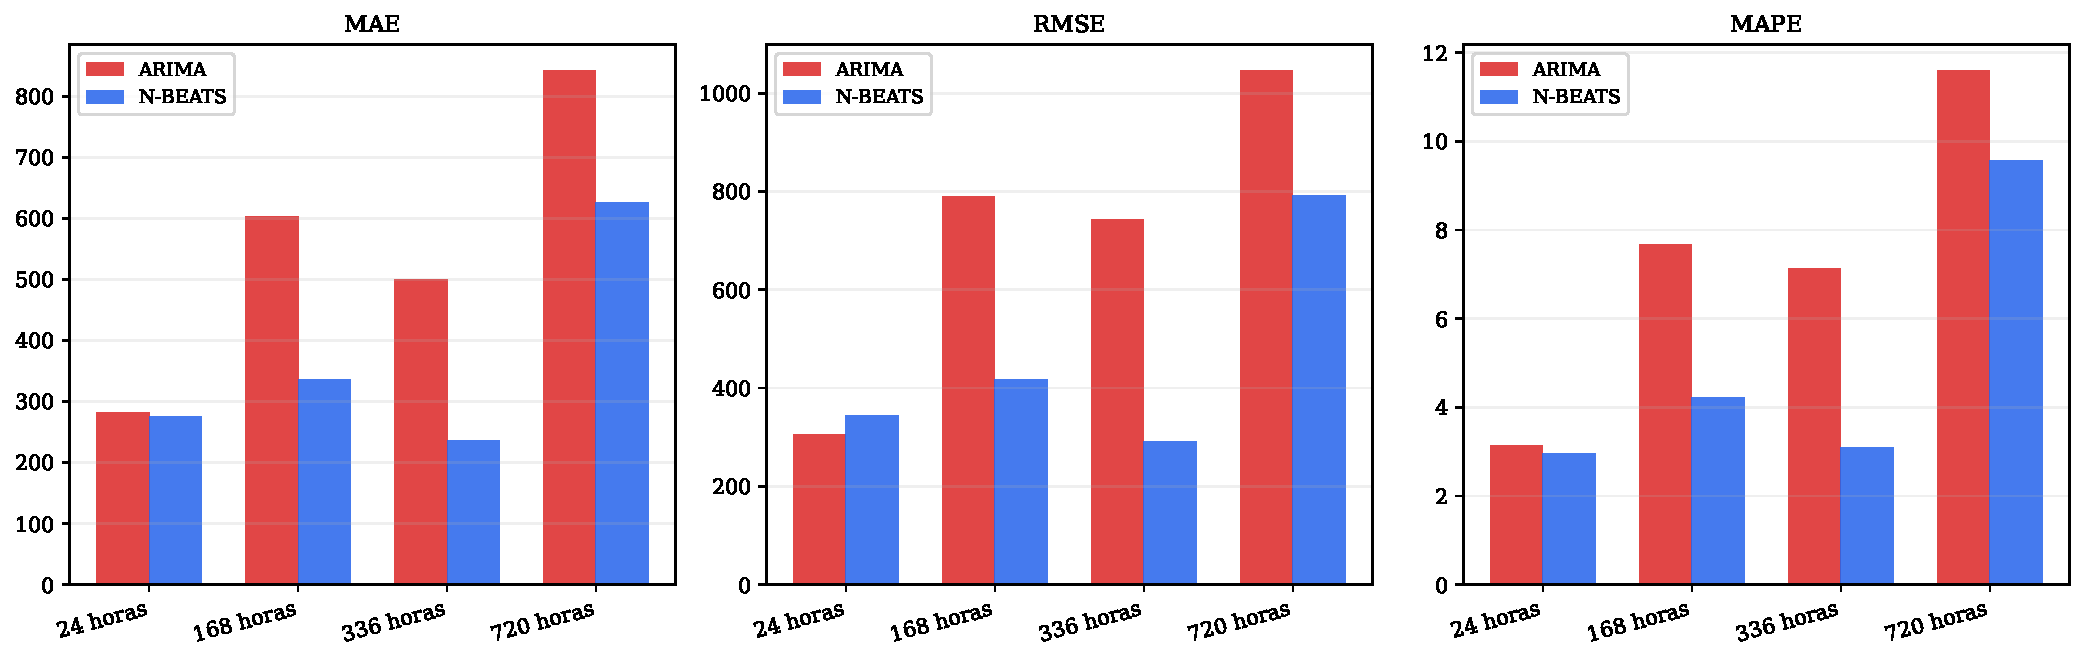
\includegraphics[width=\textwidth]{figures/metrics_comparison.pdf}
    \caption{Comparación de MAE, RMSE y MAPE entre ARIMA y N-BEATS por horizonte.}
    \label{fig:metrics-bars}
\end{figure}

\subsection{Resultados funcionales de la aplicación}

La aplicación de escritorio completó exitosamente el flujo operativo para el cual fue diseñada. La preparación del espacio de trabajo en \path{~/Energy Forecast app}, la descarga y procesamiento de datos desde Open Power System Data, la creación de modelos N-BEATS y la generación de pronósticos se verificaron mediante los cuatro modelos entrenados para la evaluación experimental. Cada modelo entrenado produjo una carpeta en \path{models/mdl\_*} con su archivo \texttt{config.json}, \texttt{metadata.json} y el registro de entrenamiento. Cada pronóstico generado quedó almacenado en una subcarpeta \path{runs/run\_*} con sus correspondientes archivos \texttt{forecast.csv}, \texttt{forecast\_input.csv} y \texttt{metadata.json}, garantizando la trazabilidad completa entre la serie de entrada, el contexto histórico utilizado y el pronóstico resultante.
